%%%%%%%%%%%%%%%%%%%% author.tex %%%%%%%%%%%%%%%%%%%%%%%%%%%%%%%%%%%
%
% sample root file for your "contribution" to a contributed volume
%
% Use this file as a template for your own input.
%
%%%%%%%%%%%%%%%% Springer %%%%%%%%%%%%%%%%%%%%%%%%%%%%%%%%%%


% RECOMMENDED %%%%%%%%%%%%%%%%%%%%%%%%%%%%%%%%%%%%%%%%%%%%%%%%%%%
\documentclass[]{svmult}

% choose options for [] as required from the list
% in the Reference Guide

\usepackage{mathptmx}       % selects Times Roman as basic font
\usepackage{helvet}         % selects Helvetica as sans-serif font
\usepackage{courier}        % selects Courier as typewriter font
\usepackage{type1cm}        % activate if the above 3 fonts are
                            % not available on your system
%
\usepackage{makeidx}         % allows index generation
\usepackage{graphicx}        % standard LaTeX graphics tool
                             % when including figure files
\usepackage{multicol}        % used for the two-column index
\usepackage[bottom]{footmisc}% places footnotes at page bottom

% see the list of further useful packages
% in the Reference Guide

\makeindex             % used for the subject index
                       % please use the style svind.ist with
                       % your makeindex program

\usepackage{amssymb}
\setcounter{tocdepth}{3}
\usepackage{amsmath}          % AMSTEX
\usepackage{amsfonts}
\usepackage{subfigure}

\usepackage{algorithm}
\usepackage{algorithmic}
\usepackage{comment}

\usepackage{url}
%\urldef{\mailsa}\path|{sandrine.mouysset, ronan.guivarch, joseph.noailles,daniel.ruiz}@enseeiht.fr|
%\urldef{\mailsb}\path|anna.kramer, leonie.kunz, christine.reiss, nicole.sator,|
%\urldef{\mailsc}\path|erika.siebert-cole, peter.strasser, lncs}@springer.com|    
%\newcommand{\keywords}[1]{\par\addvspace\baselineskip
%\noindent\keywordname\enspace\ignorespaces#1}

\begin{document}

\mainmatter

\title*{Parallel Spectral Clustering for the segmentation of cDNA Microarray Images}

\titlerunning{Parallel Spectral Clustering on cDNA Microarray Images}

\author{Sandrine Mouysset \and Ronan Guivarch \and Joseph Noailles\and Daniel Ruiz}

\institute{
Sandrine Mouysset \at  University of Toulouse - UPS - IRIT, 118 Route de Narbonne, 31062 Toulouse, France\\ \email{sandrine.mouysset@irit.fr}  \and 
Ronan Guivarch, Joseph Noailles and Daniel Ruiz  \at University of Toulouse -
INPT(ENSEEIHT) - IRIT, 2 rue
Camichel, 31071 Toulouse, France\\
\email{{ronan.guivarch,joseph.noailles,daniel.ruiz}@enseeiht.fr} 
}
%\toctitle{Lecture Notes in Computer Science}
%\tocauthor{Authors' Instructions}

\maketitle

\abstract{
Microarray technology  generates large amounts of expression level of genes to
be analyzed simultaneously.  This analysis implies microarray image
segmentation to extract the quantitative information from spots.  Spectral
clustering is one of the most relevant unsupervised method able to gather data
without a priori information on shapes or locality.  We propose  and test on
microarray images a parallel strategy for the Spectral Clustering method based
on domain decomposition and with  a criterion to determine the number of
clusters.}


% A category with the (minimum) three required fields
%\category{}{Spectral clustering}{domain decomposition}{Image Segmentation, microarray imageInformation Systems Applications}{Miscellaneous}
%A category including the fourth, optional field follows...
%\category{D.2.8}{Software Engineering}{Metrics}[complexity measures, performance measures]

%\terms{Theory}

%\keywords{Spectral Clustering, Domain Decomposition, Image Segmentation, Microarray Image} % NOT required for Proceedings
\vspace{-0.6cm}
\section{Introduction}
\vspace{-0.3cm}

Image segmentation in microarray analysis is a crucial step to extract
quantitative information from the spots \cite{rueda2009pattern},
\cite{uslan2010microarray}, \cite{giannakeas2008image}.
%  Clustering in gene-expression data sets aims to partition a data set by grouping similar elements into subsets such that each subset shares the same behaviour (for example, inhibition, repression or no expression). 
Clustering methods are used to separate the pixels that belong to the spot
from the pixels of the background and noise.  Among these, some methods imply
some restrictive  assumptions on the shapes of the spots
\cite{yang2001analysis}, \cite{rueda2005new}.  Due to the fact that the most
of spots in a microarray image have irregular-shapes, the clustering
based-method should be adaptive to arbitrary shape of spots and    should not
depend on many input parameters.  
%With these requirements, spectral clustering is considered.
Spectral methods, and in particular the spectral clustering algorithm
introduced by Ng-Jordan-Weiss \cite{speC}, are  useful when considering no a
priori shaped subsets of data. Spectral clustering exploits eigenvectors of a
Gaussian affinity matrix in order to define a low-dimensional space in which
data points can be easily clustered. But when very large data sets are
considered, the extraction of the dominant eigenvectors becomes the most
computational task in the algorithm. To address this bottleneck, several
approaches about parallel Spectral Clustering \cite{song}, %\cite{fowlkes},
\cite{Chen10} were recently suggested, mainly focused on linear  algebra
techniques to reduce computational costs. In this paper, by exploiting the
geometrical structure of microarray images, a parallel strategy based on
domain decomposition is investigated. Moreover, we propose solutions to
overcome the two main problems from the
divide and conquer strategy: the difficulty to choose a Gaussian affinity
parameter and the number of clusters $k$ which remains unknown and may
drastically vary from one subdomain to the other.
    
% The number of targeted clusters $k$ is usually assumed to be known. % 
% We investigate on %So several approaches about parallel Spectral Clustering \cite{song}, \cite{fowlkes}, \cite{Chen10} were recently suggested, mainly focused on linear  algebra techniques to reduce computational costs.
%However, the authors do not get rid of the construction of the complete affinity matrix and the problem of determining the number of clusters is still open. 

\vspace{-0.5cm}
\section{Parallel Spectral Clustering: justifications}

\vspace{-0.3cm}
\subsection{Spectral Clustering}
\vspace{-0.3cm}
Let's first give some notations and recall the Ng-Jordan-Weiss  algorithm
\cite{speC}. Let's consider a microarray image $I$ of size $l \times m$.
Assume that the number of targeted clusters $k$ is known. The algorithm
contains few steps which are described in Algorithm \ref{algo}.

\vspace{-0.2cm}
%\subsection{Algorithm}
\begin{algorithm}
\caption{Spectral Clustering Algorithm}
%\begin{algorithmic}[1]
%\begin{algorithm}
Input: Microarray image $I$, number of clusters $k$
\begin{enumerate}
\item Form the affinity matrix $A\in\mathbb{R}^{n\times n}$  with $n=l\times m$ defined by equation (\ref{defaff}).
%\begin{equation}
%A_{ir}=\begin{cases}
%\exp\left(-\frac{d\left(I_{ij},I_{rs}\right)^2}{(\sigma/2)^2}\right) \text{\  if $(ij)\neq (rs)$,}\\ \nonumber
%0 \ \text{otherwise,}
%\end{cases}
%\end{equation}
\item Construct the normalized matrix: $L=D^{-1/2}AD^{-1/2}$ with $D_{i,i}=\sum_{r=1}^{n} A_{ir} $,
\item Assemble the matrix $X=[X_1X_2..X_k]\in \mathbb{R}^{n\times k}$ by stacking the eigenvectors associated with the {$k$} largest eigenvalues of $L$,
\item Form the matrix Y by normalizing each row in the $n \times k$ matrix X,
\item Treat each row of Y as a point in $\mathbb{R}^{k}$, and group them in $k$ clusters via the {\it K-means} method,
\item Assign the original point $I_{ij}$ to cluster $t$ when row $i$ of matrix Y belongs to cluster~$t$. 
\end{enumerate}
\label{algo}
%\end{algorithmic}
\end{algorithm}
\vspace{-0.3cm}
First, the method  consists in constructing the affinity matrix based on the
Gaussian affinity measure between $I_{ij}$ and $I_{rs}$ the intensities of the
pixel of coordinates $(i,j)$ and $(r,s)$ for $i,r\in \{1,..,l\}$ and $j,s\in
\{1,..,m\}$. After a normalization step, the $k$ largest eigenvectors are
extracted. So every data point $I_{ij}$ is plotted in a spectral embedding
space of $\mathbb{R}^k$ and the clustering is made in this space by applying
K-means method. Finally, thanks to an equivalence relation, the final
partition of  data set is defined from the clustering in the embedded space.

\vspace{-0.5cm}
\subsection{Affinity measure}
\vspace{-0.3cm}

For image segmentation, the microarray image data can be considered as
isotropic enough in the sense that there does not exist some privileged
directions with very different magnitudes in the distances between points
along theses directions.  The step between pixels and brightness are about the
same magnitude. So, we can include both 2D geometrical information and 1D
brightness information in the spectral clustering method. We identify the
microarray image as a 3-dimensional rectangular set in which both geometrical
coordinates and brightness information are normalized. It is equivalent to
setting a
new distance, noted $d$, between pixels by equation (\ref{puceaff}).
So by considering the size of the microarray image, the Gaussian affinity
$A_{ir}$ is defined as follows:
\begin{equation}
A_{ir}=\begin{cases}
\exp\left(-\frac{d\left(I_{ij},I_{rs}\right)^2}{(\sigma/2)^2}\right) \text{\  if $(ij)\neq (rs)$,}\\ \label{defaff}
0 \ \text{otherwise,} 
\end{cases}
\end{equation}
where $\sigma$ is the affinity parameter and  the distance $d$ between the pixel $(ij)$ and $(rs)$ is defined by:
\begin{equation}
d\left(I_{ij},I_{rs}\right)=\sqrt{\left(\frac{i-r}{l}\right)^2+\left(\frac{j-s}{m}\right)^2+\left(\frac{I_{ij}-I_{rs}}{256}\right)^2}
\label{puceaff}
\end{equation}


This definition (\ref{puceaff}) permits a segmentation which takes into
account the geometrical shapes of the spots and the brightness information
among them. In the same way, for colored microarray images with  Cy3 and Cy5
hybridizations, we can consider 5D data with 2D geometrical coordinates and 3D
color levels.

%\subsection{Parallel Strategy}
%
%The Gaussian affinity matrix defined by (\ref{defaff}) could be interpreted as
%a discretization of the Heat kernel \cite{eigen}. And in particular, it is
%shown in \cite{icdmke} that this matrix is a discrete representation of the
%$L^2$ Heat operator onto appropriate connected domains in $\mathbb{R}^k$. By
%combining tools from Heat equations and finite elements theory, the main
%result of  \cite{icdmke} is that for a fixed data set of points, the
%eigenvectors of $A$ are the representation of functions whose support is
%included in only one connected component at once. The accuracy of this
%representation is shown, for a fixed density of points, to depend on the
%affinity parameter $\sigma$.
%From this theoretical material, the Spectral Clustering could be formulated as
%a "connected components" method in the sense that clustering in subdomains
%is equivalent in restricting the support of these $L^2$ particular
%eigenfunctions.
%So a "divide and conquer" strategy could be formulated to adapt spectral
%clustering for parallel implementation. As the main drawback of domain
%decomposition is how to ensure uniform distribution of data per processor, the
%intrinsic property of microarray image can be exploited in that respect. Due
%to the fact that microarray presents a block structure of cDNA spots, dividing
%the image in $q$ sub-images is appropriate for a domain decomposition strategy
%because it ensures a uniform distribution of data per processor.
%An overlapping interface is investigated to gather the local partitions from
%the different subdomains.
%% At the gathering level,  spectral clustering algorithm is made on a subset
%% with geometrical coordinates close to the boundaries of the previous
%% subdomains. % which geometrical coordinates are close to boundaries of
%% subdomains.
%This interface is characterized by an overlapping subset  of points whose
%geometrical coordinates are close to boundaries of neighbouring subdomains.
%This partitioning will connect together clusters which belong to different
%subdomains thanks to the following transitive relation:
%$\forall I_{i_1j_1}, I_{i_2j_2}, I_{i_3j_3} \in I$, \\
%$$
%\text{If } \ I_{i_1j_1}, I_{i_2j_2} \in C^1  \text{ and }   I_{i_2j_2}, I_{i_3j_3} \in C^2 \text{ then } $$
%\begin{equation}
% C^1 \cup C^2 = P \text{ and } I_{i_1j_1}, I_{i_2j_2}, I_{i_3j_3} \in P \label{reltrans}
%\end{equation}

%Thanks to properties of the heat equation, eigenvectors of this matrix are an asymptotical discrete representation of $L^2$ eigenfunctions with support included in only one connected component. 

\vspace{-0.5cm}
\section{Method} \label{method}
\vspace{-0.3cm}

By exploiting the block structure of microarrays, clustering can be made on
subdomains by breaking up the data set into data subsets with respect to their
geometrical coordinates in a straightforward way. With an appropriate Gaussian
affinity parameter and a method to determine the number of clusters, each
processor applies independently the spectral clustering (Algorithm \ref{algo})
on a subset of data points and provides a local partition on this data
subset.
Based on these local partitions, a grouping step ensures the connection
between subsets of data and determines a global partition thanks to the following transitive relation:
$\forall I_{i_1j_1}, I_{i_2j_2}, I_{i_3j_3} \in I$, 
\begin{equation}
\text{If } \ I_{i_1j_1}, I_{i_2j_2} \in C^1  \text{ and }   I_{i_2j_2}, I_{i_3j_3} \in C^2 \text{ then } 
 C^1 \cup C^2 = P \text{ and } I_{i_1j_1}, I_{i_2j_2}, I_{i_3j_3} \in P \label{reltrans}
\end{equation}
where $I$ is the microarray image, $C^1$ and $C^2$ two distinct clusters and
$P$ a larger cluster which includes both $C^1$ and $C^2$. We experiment this
strategy whose principle is represented in Fig.\ref{fig:principe}(a) on
several
microarray images of the Saccharomyces cerevisiae database from the Stanford
Microarray database\footnote{http://smd.stanford.edu/index.shtml}like the one
in Fig.\ref{fig:principe}(b).
%The clustering result on a $4 \times 2$ greyscaled spotted of this microarray
%image  is plotted in figure \ref{fig:puzzle} (a)-(b).

\begin{figure}
  \begin{center}
    %\subfigure[Principle of parallel spectral clustering.]
    {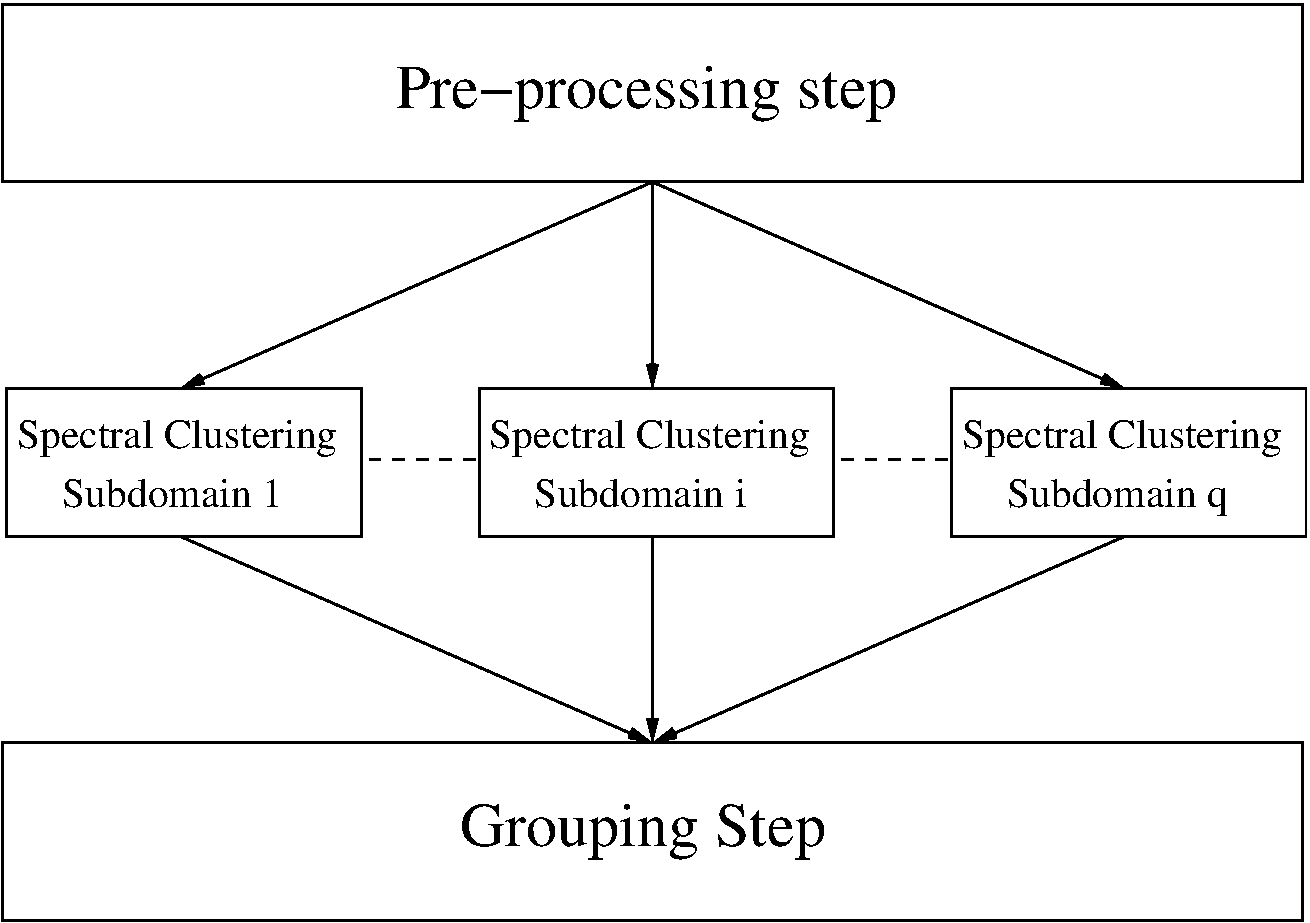
\includegraphics[width=0.40\linewidth]{intersectionq}}
    \hspace{1cm}
    %\subfigure[Block structure of microarray image]
    { {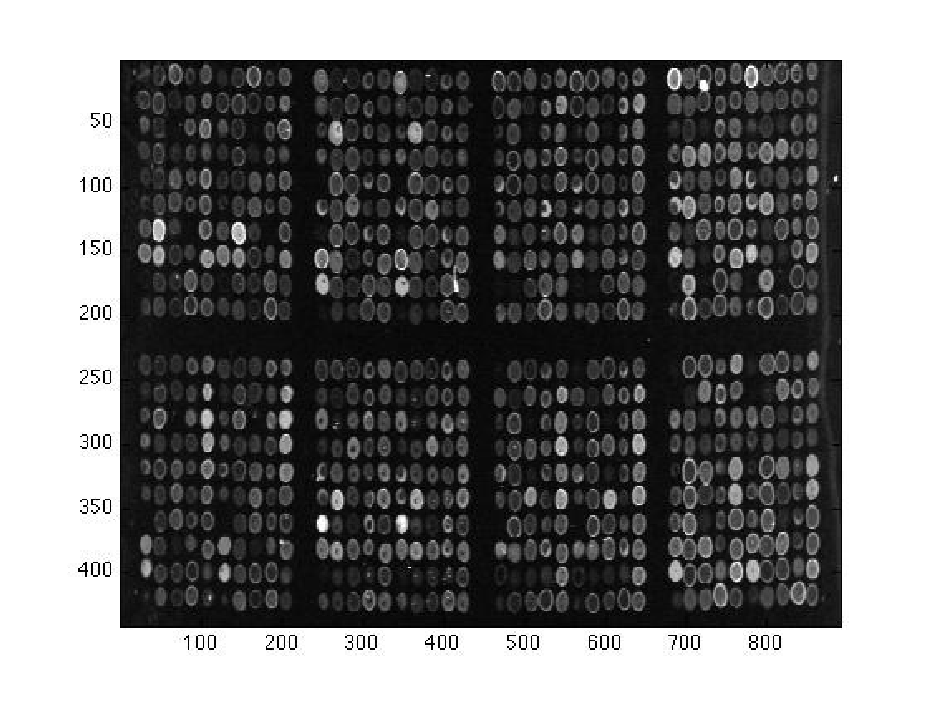
\includegraphics[width=0.40\linewidth]{pucegris}}}
  \end{center}
  \caption{Principle of the parallel strategy for microarray image : (a) Principle of parallel spectral clustering and (b) Block structure of microarray image.}
  \label{fig:principe}
\end{figure}

It is important to see how the parallel approach can take advantage of the
specificities of this particular application. Indeed, when splitting the
original image into overlapping sub-pieces of images, the local spectral
clustering analysis of each sub-piece involves the creation of many affinity
matrices of smaller size. The total amount of memory needs for all these
local matrices is much less than the memory needed for the affinity matrix
covering the global image.
% (it is marginally larger than the equivalent of a
%block diagonal splitting of the global matrix, simply because of the
%overlapping areas between sub-images).
%As opposed to some sparsification of the global affinity matrix %(which can
%%still be also exploited on each of the sub-ma\-tri\-ces, for further
%%computation cost reduction) 
%there is no need to build every entry and zero
%some of these afterwards, parallelism is straightforward without the need to
%identify structures in the graph of the sparsified global affinity matrix,
%and global coherence in the final results is fully ensured (without any
%aspects of approximation theory)  because of the grouping step based
%on the overlapping areas.
Additionally, the analysis of each subproblem is made from the extraction of
eigenvectors in the scaled affinity sub-matrices, keeping in mind that one
eigenvector is needed for each identified cluster in the corresponding
sub-image. 
In that respect, the parallel approach enables us to decrease
drastically the cost of this eigenvector computation.
%because each subproblem
%will include a number of clusters less than three times the number of spots
%covered by each sub-image (much less than the total number of clusters in the
%global image) and, on top of that, the sum of the dimensions of these
%eigenvectors is only marginally greater (again, because of the overlapping
%areas between sub-images) than the total dimension of the global affinity
%matrix.

%Finally, if one could ensure that the spots are regularly distributed in the
%spotted microarray image and can be easily separated in sub-images, %(this seems
%%natural, but not so straightforward to determine in a simple and generic
%%manner, as one can see in Fig.\ref{fig:principe}(b)), 
%it may even be possible
%to avoid the overlapping areas and the grouping step, resulting in a fully
%parallel scheme with easy control of the parameters and gains in memory and
%computations.

\vspace{-0.5cm}
\subsection{Choice of the affinity parameter}
\vspace{-0.3cm}

The Gaussian affinity matrix is widely used and depends on a free parameter
which is the affinity parameter, noted $\sigma$, in equation (\ref{defaff}). It
is known that this parameter conditions the separability between clusters in spectral embedding space and affects the results. 
A global heuristics for this parameter was proposed in
\cite{vec08b} in which both the dimension of the problem as well as the
density of points in the given p-th dimensional data set are  integrated. With
an assumption that the 
%$p$-dimensional 
data set is isotropic enough, the image
data set $I$ is included in a $p$-dimensional box bounded by $D_{max}$ the
largest distance $d$ (defined by (\ref{puceaff})) between pairs of points in
$I$:
$$\displaystyle 
D_{\max} = \max_{ \stackrel{1\leq i,r \leq l}{1\leq j,s \leq m} }
d(I_{ij},I_{rs}).$$
%,$ where $d$ is the distance defined by equation
%(\ref{puceaff}).
%By considering an uniform distribution in which all pair of data points are
%separated by the same distance, a reference distance is  defined.
A reference distance 
%defined by (\ref{sigma})
which represents the distance in
the case of an uniform distribution is defined as follows:
% in the sense that all pairs of
%points in such distribution are separated by the same distance:
%this distance represents .% in the box of edge size the maximum  of the
%Euclidean norm between data points.%$D_{max} = \max_{1\leq i,j \leq n}  \|
%x_i - x_j \|$.
\begin{equation}
 \sigma = \frac{D_{\max}}{n^{\frac{1}{p}}}, \label{sigma}
\end{equation}
in which $n=l\times m$ is the size of the microarray image and  $p=3$ (resp.
$p=5$) with 2D geometrical coordinates and 1D brightness (resp. 3D color).
From this definition, clusters may exist if there are points that are at a
distance no more than a fraction of this reference distance $\sigma$.
%points are at least distanced by a fraction of $\sigma$.  
This global parameter is defined with the whole image data set $I$ and gives a
threshold for all spectral clustering applied independently on the several
subdomains.
%$\sigma$ will be fixed for each subset  the threshold on the union of subdomains. 
%We could define such parameter for each subdomain. However, with a
%straightforward decomposition as the one proposed, one can find easily that a
%local $\sigma_{l}$ in each subdomain will be close to the value of a global
%$\sigma$ defined on the whole data set in the same way.

\vspace{-0.7cm}
\subsection{Choice of the number of clusters}
\vspace{-0.3cm}

The problem of the right choice of the number of clusters $k$ is crucial.
%because this number may vary from one subdomain to the other in such
%a domain decomposition strategy.
We therefore consider in each subdomain a
quality measure based on ratios of Frobenius norms, see for instance
\cite{vec08b}. After indexing data points per cluster for a value of $k$, we
define the indexed affinity matrix whose diagonal affinity blocks
represent the affinity within a cluster and the off-diagonal ones the
affinity between clusters Fig.\ref{fig:sparseaff}(a).
The ratios, noted $r_{ij}$, between the Frobenius norm of the off-diagonal
blocks $(ij)$ and that of the diagonal ones $(ii)$ could be evaluated.  %By
%definition, the appropriate number of clusters, noted $\hat{k}$, corresponds to a
%situation where points which belong to different clusters have low affinity
%between each other whereas points in same clusters have higher affinity.
Among various values for $k$, the final number of cluster is defined so that
the affinity between clusters is the lowest and the affinity within cluster
is the highest:
\begin{equation}
\hat{k} = argmin \sum_{i\neq j} r_{ij}. \label{clusk}
\end{equation} 
Numerically, the corresponding loop to test several values of $k$ until
satisfying (\ref{clusk}) is not extremely costly but only requires to
concatenate eigenvectors, apply K-means, and a reordering step on the affinity
matrix to compute the ratios.  Furthermore, this loop becomes less and less
costly when the number of processors increases. This is due to the fact that
eigenvectors become much smaller with affinity matrices of smaller size. Also,
subdividing the whole data set implicitly reduces the Gaussian affinity to
diagonal subblocks (after permutations).
For the $4 \times 2$ greyscaled spotted microarray image which corresponds
to one subdomain, the original data set and its clustering result are plotted in
Fig.\ref{fig:sparseaff}(b) for $k=8$.
\begin{figure}
  \begin{center}
%     \setlength{\unitlength}{5mm}
   % \subfigure[Block structure of the indexed affinity matrix for $k=8$.]
    {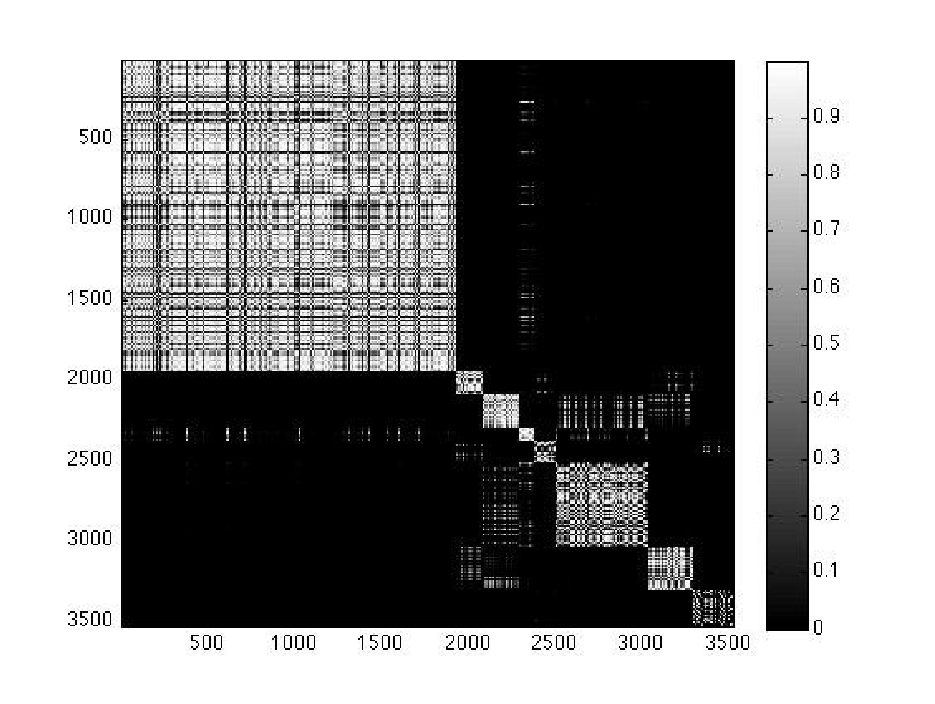
\includegraphics[width=0.4\linewidth]{Aindexk8}}
%  {\includegraphics[width=0.45\linewidth]{spy_Aord_k5}}
    \hspace{0.2cm}
   %\subfigure[Original data and its clustering result.]
   {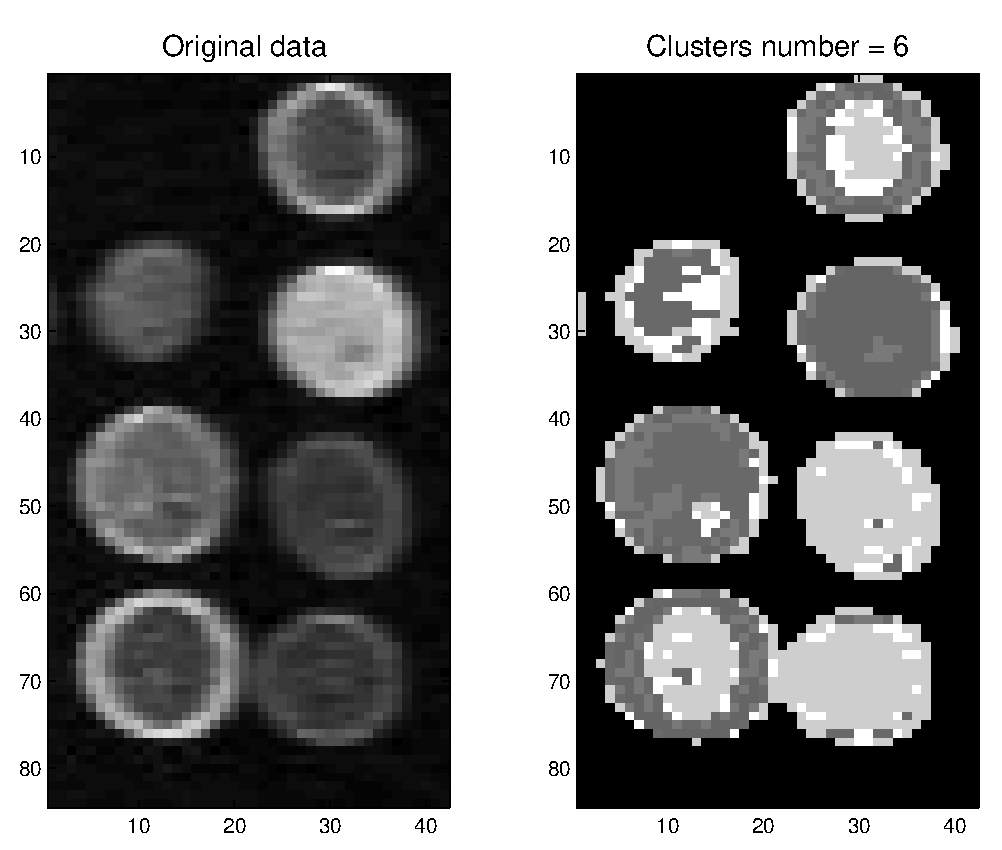
\includegraphics[width=0.35\linewidth]{Onesubdomain}}
 \end{center}
\caption{Clustering on one sub-domain made by $4 \times 2$ greyscaled spotted
microarray image (3500 pixels): (a) Block structure of the indexed affinity
matrix for $k=8$ and (b) Original data and its clustering result.}  
\label{fig:sparseaff}
\end{figure}

\vspace{-1.1cm}
\subsection{Parallel Implementation of the Spectral Clustering Algorithm}
\vspace{-0.3cm}

The FORTRAN 90 implementation of the parallel Spectral Clustering Algorithm
follows the Master-Slave paradigm with the MPI library to perform the
communications between processors (algorithms \ref{algo-slave} and \ref{algo-master}).
\begin{comment}
Some points have to be precised.
\begin{enumerate}
\item {\it Pre-processing step: Partition  $S$ in $q$ subdomains :}
%The whole data set is subdivided in $q$ subboxes which have a non-empty
%intersection. The width of the overlapping is given as a parameter of the
%algorithm.
The affinity parameter $\sigma$ is computed with the formula (\ref{sigma}).
Then the bandwidth of the overlapping is function of this distance reference
$\sigma$ and is fixed to $3\times \sigma$.
\item {\it Communications}
The communications between the Master and the Slaves are performed using
classical MPI primitives as \textsc{Mpi\_Send} and \textsc{Mpi\_Recv}.
\item {\it Spectral Clustering Algorithm}
\begin{itemize}
%\paragraph{Computation of the spectrum of the affinity matrix (\ref{defaff})}
  \item {Computation of the spectrum of the affinity matrix (\ref{defaff}):}
        classical routines from LAPACK library \cite{anderson1999lapack} are used to
        compute selected eigenvalues and  eigenvectors of the normalized  affinity
        matrix $A~$ for each subset of data points.
  \item {Number of clusters:}
        %\paragraph{Number of clusters}
        the number of clusters $k$ is chosen to satisfy (\ref{clusk}).
  \item {Spectral embedding:}
        %\paragraph{Spectral embedding}
        the centers for K-means initialization in the spectral embedding are
        chosen to be the furthest from each other along a direction.
\end{itemize}
\item {\it Grouping step} This step is  made using the transitive relation (\ref{reltrans})
\end{enumerate}
%The final partition is formed by grouping partitions from the $q$ independent
%spectral clustering analyses.  The grouping step is made using the transitive
%relation (\ref{reltrans}).  If a point belongs to two different clusters, both
%clusters are then included in a larger one.  For example, for $q=2$, the
%connection between clusters of two adjoint partitions is achievable thanks to
%the overlap between the two corresponding subdomains.
As output of the parallel method, a partition of the whole data set $S$ and
the final number of clusters $k$ are given.
We given this Master-Slave implementation in the algorithms
\ref{algo-slave} and \ref{algo-master}.
\end{comment}

\begin{algorithm}
\caption{Parallel Algorithm: Slave}
\label{algo-slave}
\begin{algorithmic}[1]
%\begin{algorithm}
  \STATE Receive the sigma value and its data subset from the Master
         (\textsc{Mpi\_Recv})
  \STATE Perform the Spectral Clustering Algorithm on its subset
  \STATE Send the local partition and its number of clusters to the Master
         (\textsc{Mpi\_Send})
\end{algorithmic}
\end{algorithm}

\begin{algorithm}
\caption{Parallel Algorithm: Master}
\label{algo-master}
\begin{algorithmic}[1]
%\begin{algorithm}
  \STATE Pre-processing step\\
        \hspace{0.3cm} 1.1 Read the global data and the parameters\\
        \hspace{0.3cm} 1.2 Split the data into subsets regarding the geometry\\
        \hspace{0.3cm} 1.3 Compute the affinity parameter $\sigma$\\
  \STATE Send the sigma value and the data subsets to the other processors
         (MPI CALL)
  \STATE Perform the Spectral Clustering Algorithm on subset 1
  \STATE Receive the local partitions and the number of clusters from each
         processor (MPI CALL)
  \STATE Grouping Step\\
         \hspace{0.3cm} 5.1 Gather the local partitions in a global
                        partition thanks to the transitive relation\\
         \hspace{0.3cm} 5.2 Give as output a partition of the whole data
                        set $S$ and the final number of clusters $k$
\end{algorithmic}
\end{algorithm}

%\pagebreak[4]

\vspace{-0.7cm}
\section{Numerical Experiments} \label{numerical}
\vspace{-0.3cm}

The numerical experiments were carried out on the Hyperion
supercomputer\footnote{http://www.calmip.cict.fr/spip/spip.php?rubrique90} of the CICT.
%Hyperion is the latest supercomputer of the CICT (Centre Interuniversitaire de
%Calcul de Toulouse). With its 352 bi-Intel "Nehalem" EP quad-core nodes it can
%develop a peak of 33TFlops. Each node has 4.5 GB memory dedicated for each of
%the cores and an overall of 32 GB fully available memory on the node that is
%shared between the cores.
For our tests, the domain is successively divided in $q=\{18,32,45,60,64\}$
subboxes.
The timings for each step of parallel algorithm are measured. We test this
Parallel Spectral Clustering on one microarray image from the Stanford
Microarray Database.
For a decomposition in 64 subboxes, the clustering result is plotted in
Fig.\ref{biopuceresult}. The original microarray image of 392931 pixels which
represents 8 blocks of 100 spots is plotted on the left of the figure.
After the grouping step, the parallel spectral clustering result has
determined 11193 clusters which are plotted on the right of
Fig.\ref{biopuceresult}.
Compared to the original data set, the shapes of the various hybridization
spots are well described.
\vspace{-0.3cm}
\begin{table}
\caption{Microrarray image segmentation results for different splittings.} \label{biopuce_res}
\begin{center}
\begin{tabular}{p{1.5cm}p{1.5cm}p{1.5cm}p{1.7cm}p{1.5cm}p{1.5cm}p{1.7cm}}
\hline\noalign{\smallskip}
Number & Number & Time & Time & Time & Total & Memory \\
of proc. & of points & $\sigma$ & parallel SC & Grouping & Time & Cons.\\
\noalign{\smallskip}\svhline\noalign{\smallskip}
18 & 22000 & 1413 & 36616 & 892 & 38927 & 7.75\\
32 & 12500 & 1371 & 7243  & 794 & 9415  & 2.50\\
45  & 9000  & 1357 & 2808  & 953 & 5127 & 1.30\\
60  & 6800  & 1360 & 1153  & 972 & 3495 & 0.74\\
64 & 6300  & 1372 & 1030  & 744 & 3157  & 0.64\\
\noalign{\smallskip}\hline\noalign{\smallskip}
\end{tabular}
\end{center}
\end{table}
\vspace{-0.3cm}

We give in Table \ref{biopuce_res}, for each distribution, the number
of points on each processor, the time in seconds to compute $\sigma$ defined by
(\ref{sigma}), the time in the parallel Spectral Clustering step, the time of
the grouping phase, the total time and the memory consumption in GigaOctets.
%All times are given in seconds.
\begin{figure}
   \begin{center}
 {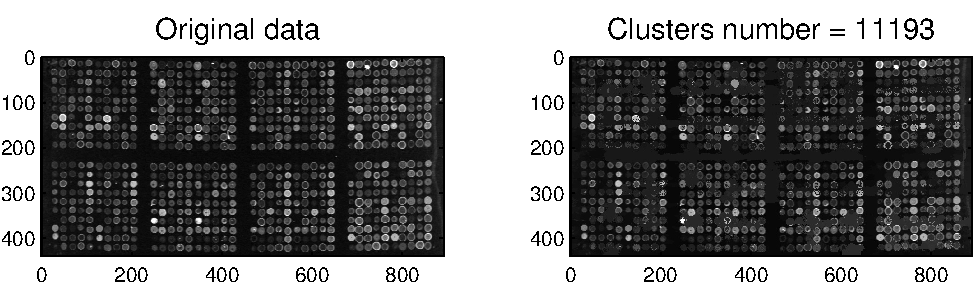
\includegraphics[width=\linewidth]{biopuce250b}}
   \end{center}
   \caption{Original microarray image and its clustering result.}  
   \label{biopuceresult}
 \end{figure}
%The number of processors corresponds to various splittings where we try to
%have as much squared subdomains as possible. Because the microarray image has
%twice more points in a direction than in the other, we have the following
%processor repartitions: $18 = 3\times6$, $32 = 4\times8$, $45 = 5\times9$,
%$60 = 6\times10$ and $64 = 8 \times 8$. The exception is the last splitting
%where we take the maximum number of processors that are available (64
%processors in these experiments).

%Note that we cannot take less than 18 processors: with less processors, the
%number of points by subset and consequently the memory needed on each processor
%exceeds the memory capacity of each processor.
The first remark is that the total time decreases drastically when we increase
the number of processors. Logically, this is time of the parallel part of the
algorithm (step 3.) that decreases while the two other steps (1 and 5),
that are sequential, remain practically constant.

%\paragraph{Parallel part}
To study the performance of our parallel algorithm, we compute the speedup.
%for the different numbers of processors.
Because we cannot have a result with only
one processor in order to have a sequential reference (lack of memory), we
take the time with the 18 processors, the minimum number of processors in
order to have enough memory by processor. The speedup for $q$
processors will then be defined as $S_q = \frac{T_{18}}{ T_q}.$
%we plot in Fig.\ref{fig:costs}(a) these speedups.

%\begin{figure}
 %  \begin{center}
  %   \setlength{\unitlength}{5mm}
 %{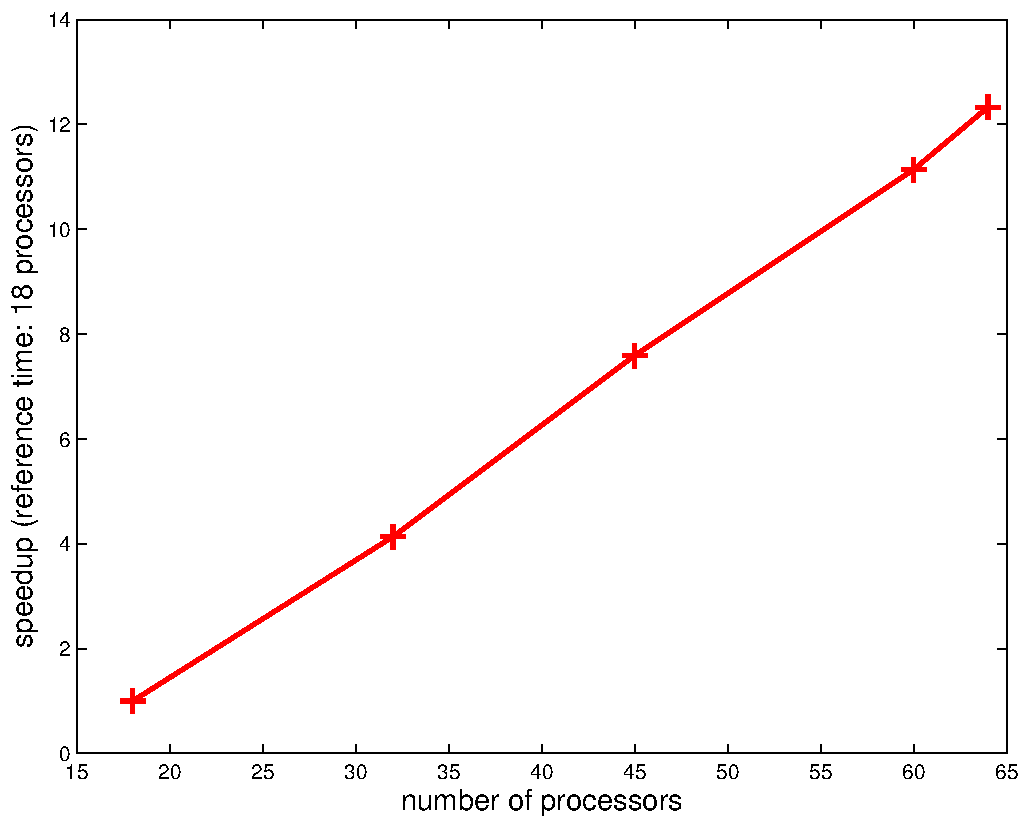
\includegraphics[width=0.6\linewidth]{speedup}}
  % \end{center}
  % \caption{Speedup with the 18 processors time as reference}  
  % \label{fig:speedup}
 %\end{figure}

We can notice in Fig.\ref{fig:costs}(a)  that the speedups increase faster than the number of processors:
for instance, from 18 to 64 processors, the speedup is 12 although the number
of processors grows only with a ratio $3.55$. This good performance is confirmed if we draw the mean computational costs per
point of the image.We define, for a given number of processors, the parallel computational cost
(resp. total computational cost) the time spent in the parallel part (parallel
Spectral Clustering part) (resp. total time) divided by the average number of
points on each subdomain. We give in Fig.\ref{fig:costs} (b), these parallel
(plain line) and total (dashed line) computational costs.

\begin{figure}
  \begin{center}
    %\subfigure[Speedup with the 18 processors time as reference]
    {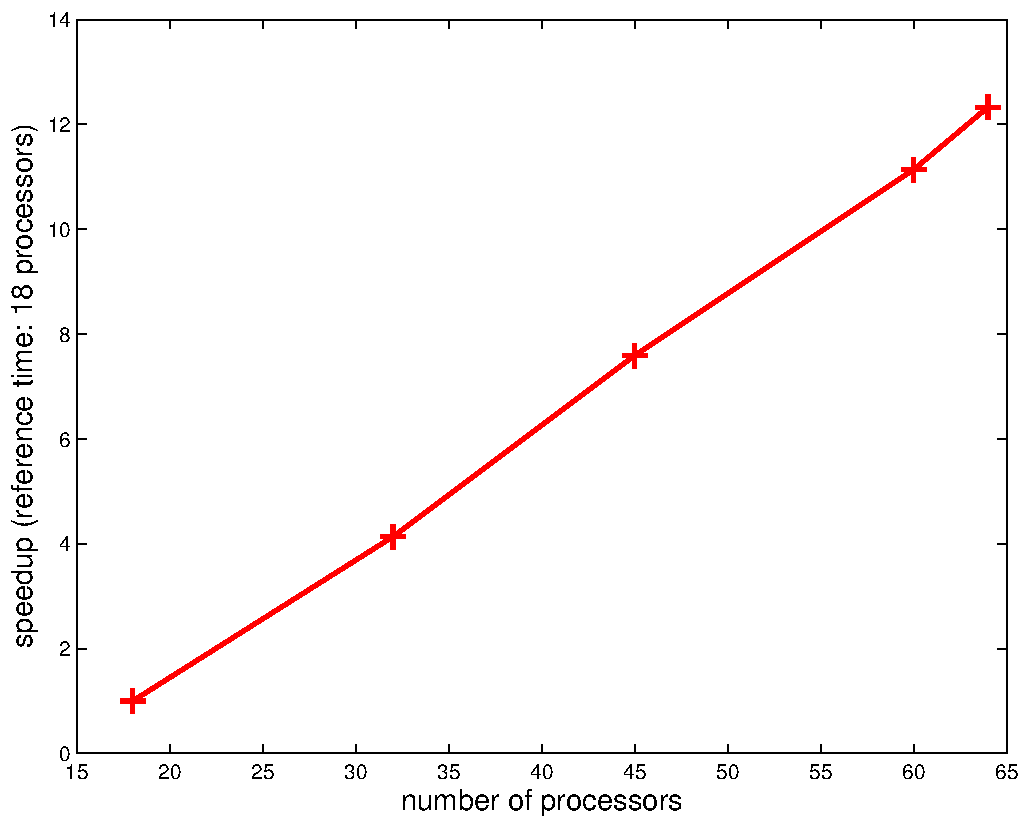
\includegraphics[width=0.35\linewidth]{speedup}}
    \hspace{2cm}
    %\subfigure[Parallel and total computational costs] 
    {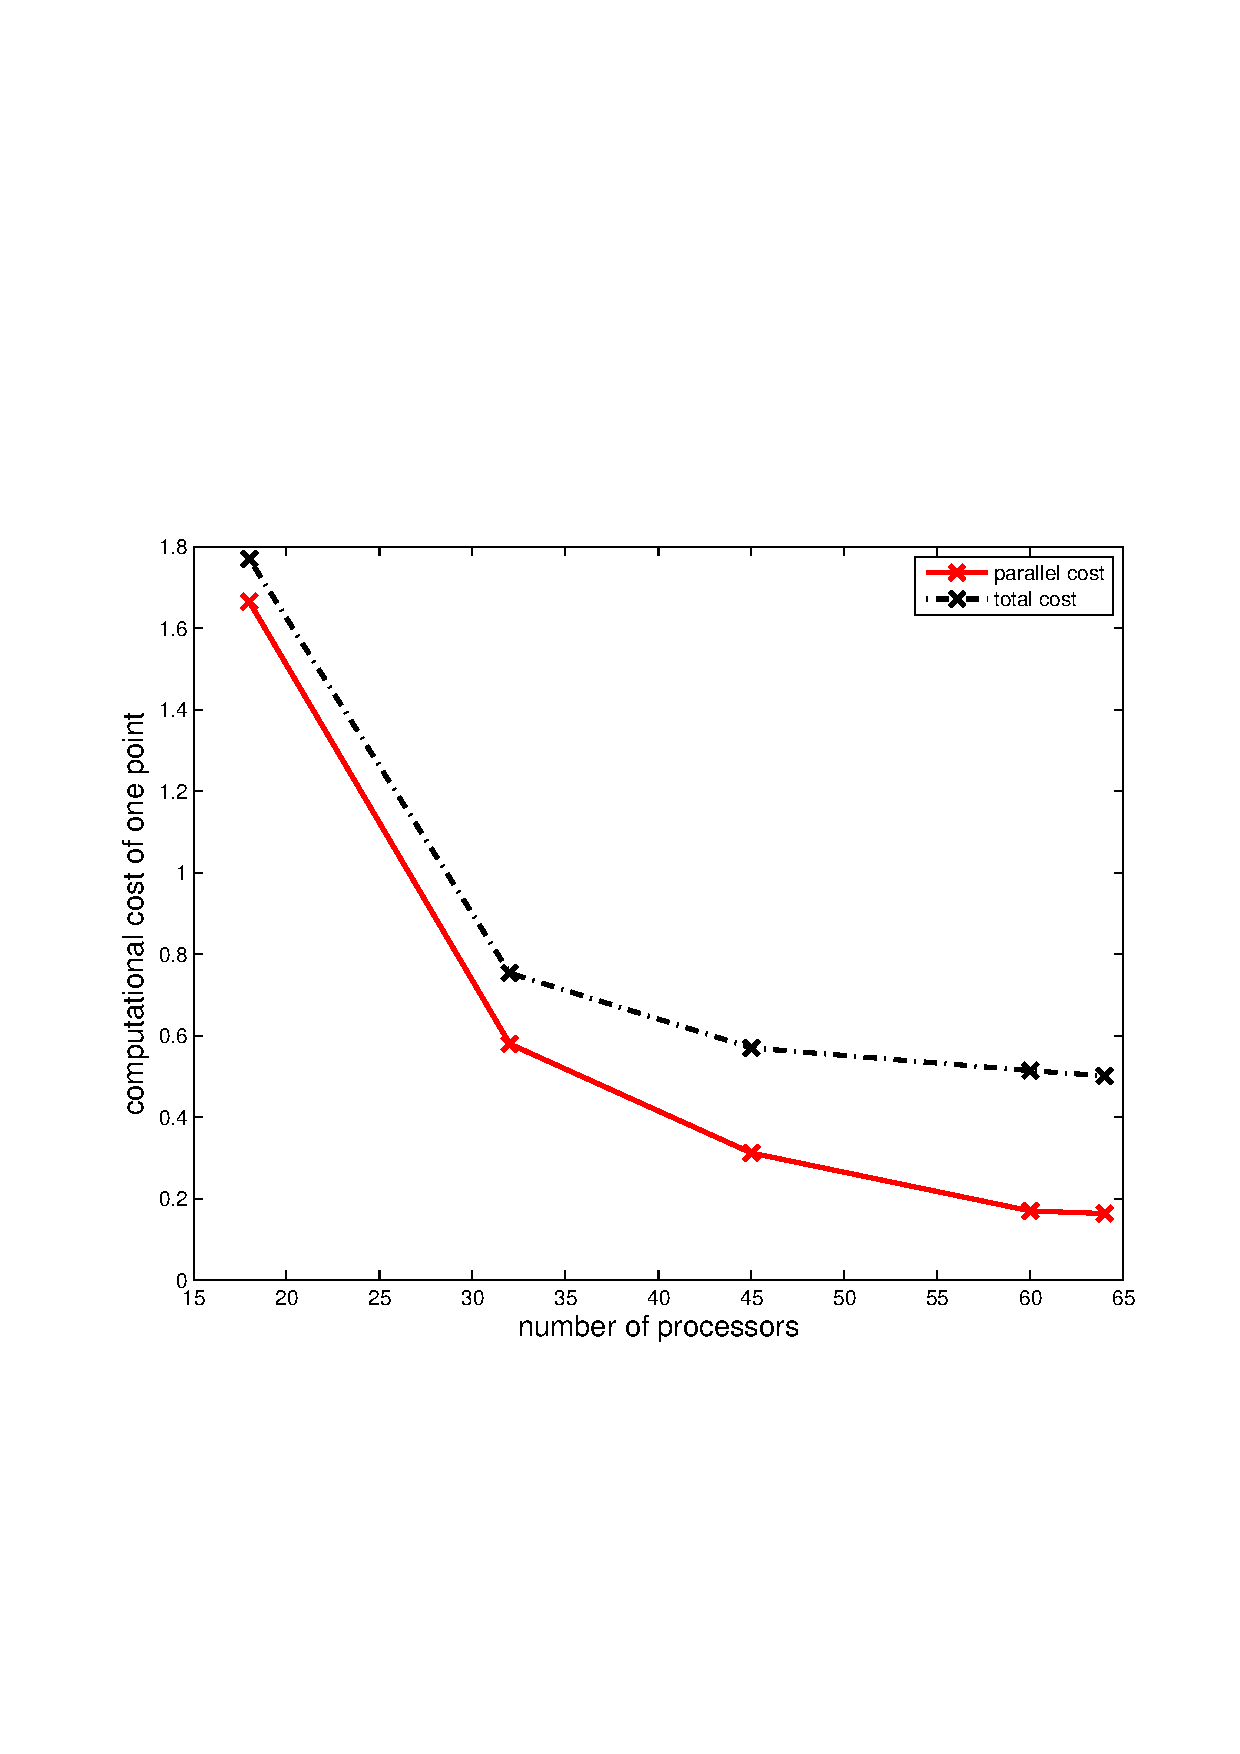
\includegraphics[width=0.35\linewidth]{cost}}
  \end{center}
  \caption{Performances of the parallel part : (a) Speedup with the 18
  processors time as reference and (b) Parallel and total computational
  costs.}
  \label{fig:costs}
 \end{figure}

We can observe from Table 1 that the less points we have by subset, the faster
we go and the decreasing is better than linear. This can be explained by the
non-linearity of our problem which is the computation of eigenvectors from the
Gaussian affinity matrix. There are much better gains in general when smaller
subsets are considered.

%\paragraph{Sequential parts}
%We can add that this good performance with a large number of processors is
%penalized by the sequential parts. Indeed the times spent in these parts
%depend of the global number of points of the image and of the number of
%computed clusters. In our example they remain practically 
%constant. As opposed to previous results with smaller images, the
%time of the sequential computations are not negligible:
%\begin{itemize}
%  \item for example with 64 processors, the time for computing the $\sigma$
%        parameter is greater than the time spent in the Spectral Clustering
%        itself;
%  \item the grouping step time that depends of the number of computed clusters
%        is also important in our example.
%\end{itemize}
%The computation of the $\sigma$ parameter could easily be parallelized. This
%is a maximum search over distances between pixels. The computation of these
%independent distances could be done in parallel,  local maximum could be found
%and a reduce MPI operation of these maximums would give us the $\sigma$
%parameter. This is a part to develop.
%Because it is a global operation, the grouping step (define the final global
%clusters from the local partial clusters) seems more difficult to parallelize.
%A good solution to minimize the time spent in this part would be the fully
%parallel scheme specific to this particular application, mentioned at the end
%of the introduction of section \ref{method} where the spotted microarray image
%is separated in sub-images. In this case, we would only consider the parallel
%Spectral Clustering of independent sets of spots; when doing so, we may expect
%to obtain a small number of partial clusters, fast to group in global
%clusters.

\vspace{-0.7cm}
\section{Conclusion}
\vspace{-0.3cm}

With the domain decomposition strategy and heuristics to determine the
choice of the Gaussian affinity parameter and the number of clusters, the
parallel spectral clustering becomes robust for microarray image segmentation
and combines intensity and shape features. The numerical experiments show the good behaviour of our parallel strategy
when increasing the number of processors and confirm the suitability of our
method to treat microarray images. 

However, we find two limitations: the lack of memory when the subset given to
a processor is large and the time spent in the sequential parts which stays
roughly constant and tends to exceed the parallel time with large number of
processors. 
To reduce the problem of memory but also to reduce the spectral clustering
time, we can study some techniques for sparsifying the Gaussian affinity
matrix: some sparsification techniques, such as thresholding the affinity
between data points, could also be introduced to speed up the algorithm when
the subdomains are still large enough. With sparse structures to store the
matrix, we will also gain a lot of memory.  However, we may have to adapt our
eigenvalues solver and use for example ARPACK library
\cite{lehoucq1998arpack}.
%Moreover, due to the principle of the
%parallelization strategy, an implementation via GPU is possible.
To reduce the time of the sequential parts, we could investigate parallelization of the
computation of the $\sigma$ parameter and ability to separate the spotted
microarray image in sub-images. 
%have to study the suggested solutions at the end of section \ref{numerical}: parallelization of the
%computation of the $\sigma$ parameter and ability to separate the spotted
%microarray image in sub-images.
%Separate the spotted microarray image is a promising solution. Using the
%gridding structure of the image, we could benefit from two possibilities of
%parallelism: fully parallel scheme at the level of the image and the parallel
%Spectral Clustering algorithm we develop for each sub-image (single spot or
%set of spots). Our future works will investigate these issues.
\vspace{-0.8cm}
\small{
\bibliographystyle{abbrv}
\bibliography{moi}
}
\end{document}
